\documentclass{article}
\usepackage{natbib}
\usepackage{hyperref}
\usepackage{graphicx}
\usepackage{subcaption}
\usepackage{amssymb,amsmath,amsthm}
\usepackage{xcolor}
\usepackage{xspace}
\usepackage[nameinlink,capitalize]{cleveref}

\newcommand{\fady}[1]{\textcolor{cyan}{$\langle${\slshape{\bfseries Fady:} #1 }$\rangle$}}
\newcommand{\Rnum}{\mathcal{R}_0}
\theoremstyle{definition} % amsthm only
\newtheorem{proposition}{Proposition}
\newtheorem{theorem}{Theorem}

\bibliographystyle{apalike}

\title{Testing and Isolation Efficacy; Insights from a Simple Epidemic Model }

\begin{document}
\maketitle

% %%%%%%%
\section{Introduction}

One of the real chalanges interpreting COVID-19 dynamics is to unravel/investigate information gained from data. One of the strongest singnals we get to see is the daily case reports which are driven by a combination of two processes: (i) epidemic processes and (ii) testing processes. The real chalange here is to seperate these two processes. Simple mathematical models have a long history in providing useful insights facing with real epidemiological chalanges \citep{ross1911prevention} [maybe add influenza work, ideas?]. We developed a model to incorporate mechanistic processes of epidemic processes and testing. We used the model to study the potential effect of testing strategies and slow-fast reporting testing result. 

There are different testing strategies with test-specific efficacy, the time required for the results to be reported and the cost of the test. Testing strategies can be grouped into two broad cathegories including (i) random testing across the whole population and (ii) Non-random/bios testing. Note that contact tracing is an example of non-random testing strategies. Each of these strategies has been used as a tool to study COVID-19; see (refs) for group (i) and (refs) for group (ii). The advantage of non-random testing comparing to random testing has been investigated specifically during COVID-19 pandemic (refs). Further, lots of efforts have been invested in developing widely accessible and fast tests in order to metigate the spread of the pandemic (refs). As a comparison of slow versus fast test, the viral PCR test, which is the most accessible test and takes about four days, is very slow relative to the potential tests such as breath-based test \citep{ruszkiewicz2020diagnosis}, which is still in trial stage and takes a few seconds. The point to be made is that there can be a potential advantage of slow test.

In this work we developed a model to incorporate epidemic processes and testing processes mechanisticly to study the potential effect of testing strategies and slow-fast testing. The analysis of the deterministic model included deriving the basic reproduction number, $\Rnum$, as the index of threshold dynamics and the effect of underlying parameters on this key index. We found that the non-random testing strategy is more effective than the random testing. Specifically, the required critical testing intensity to keep $\Rnum$ lower than the threshold value of one, is much lower in the non-random testing than the random one. Further, we show that there is a potential advantage of slow reporting of test result on the spread of the infection.  


% %%%%%%%
\section{Method}

We used a SIR (Susceptible-Infectious-Recovered) deterministic model. In order to collect cumulative reported negative or positive tests, two 'integrator' or 'accumulator' compartments, $N$ and $P$, were incorporated. The flowchart is 

\begin{figure}[!h] 
\begin{center} 
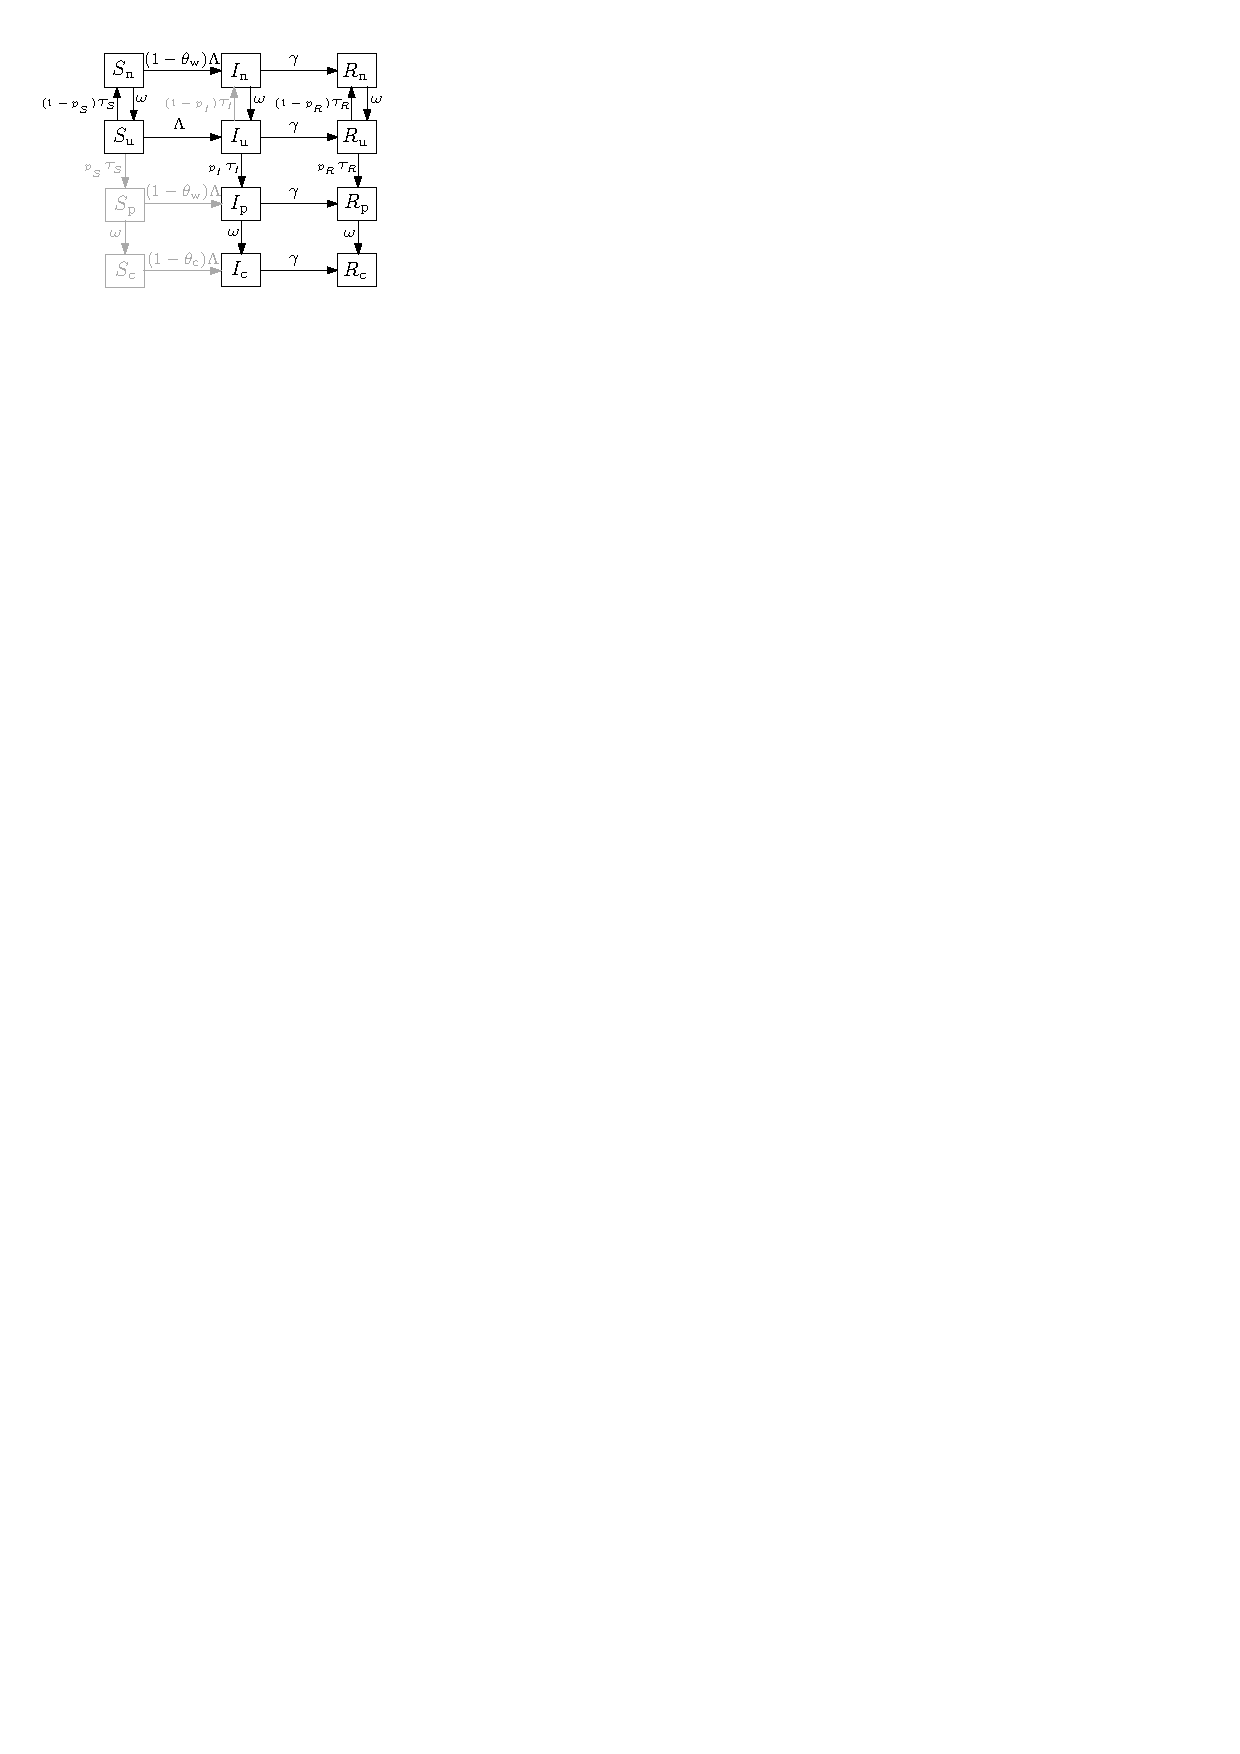
\includegraphics[scale=0.3]{./pix/sir_comp.png}
\caption{\small Flowchart of the SIR (Susceptible-Infectious-Recovered) model. Say more here to make it stand on its own.
\label{fig:flowchart}} 
\end{center} 
\end{figure}

The model is
\begin{align}
\label{model}
 d S_u/dt &= -\Lambda S_u - F_S S_u + \omega S_n \\
 d S_n/dt &= -\Lambda S_n + (1-p_S) F_S S_u - \omega S_n \\
 d S_p/dt &= -\Lambda S_p + p_S F_S S_u - \omega S_p \\
 d S_t/dt &= -\Lambda S_t + \omega S_p \\
 d I_u/dt &= \Lambda S_u - F_I I_u + \omega I_n  - \gamma I_u  \\
 d I_n/dt &= \Lambda S_n + (1-p_I) F_I I_u - \omega I_n -\gamma I_n \\
 d I_p/dt &= \Lambda S_p + p_I F_I I_u - \omega I_p -\gamma I_p \\
 d I_t/dt &= \Lambda S_t + \omega I_p - \gamma I_t  \\
 d R_u/dt &= \gamma I_u - F_R R_u + \omega R_n \\
 d R_n/dt &= \gamma I_n + (1-p_R) F_R R_u - \omega R_n  \\
 d R_p/dt &= \gamma I_p + p_R F_R R_u  - \omega R_p  \\
 d R_t/dt&= \gamma I_t + \omega R_p  \\
 dN/dt &= \omega (S_n + I_n + R_n)   \\
 dP/dt &= \omega(I_p + R_p),
\end{align}

where $\beta$, (1/day), is the disease transmission rate, $\eta_w$ and $\eta_t$ are the isolation parameters for awaiting and reported individuals, respectively, $\Lambda$ is the force of infection and defined as 
\begin{equation}
\label{Lambda}
\Lambda=\beta \frac{(I_u+\eta_w I_n+\eta_w I_p+ \eta_t I_t)}{N_0},
\end{equation}
where $N_0$ is the total population size. Further, $\omega$, (1/day), is the rate of onward flow from the awaiting positive or negative compartments to reported or untested compartments, respectively, $\gamma$, (1/day), is the recovery rate, $\rho$, (1/day), is the per capita testing intensity across the whole population. Further, various testing strategies are incorporated through the compartment-specific relative testing weights $W_S$, $W_I$ and $W_R$. The weighted number of people available for tests is defined as $W = W_S S_u + W_I I_u + W_R R_u$, and the scaling parameter for testing defined as \begin{equation}
\label{sigma}
\sigma = \frac{\rho N_0}{W}.
\end{equation}
Thus, the weighted testing rate is defined as $F_Z=\sigma W_Z$, for $Z \in \{S,I,R\}$. 

- In this model we assumed: (i) all groups being exposed to all others, (ii) there is a single force of infection, $\Lambda$, that is, where a susceptible individual move to does not depend on who infected it, (iii) a perfectly specific test, $p_S=0$, for simplicity in analysis, (iv)  $\eta_t \leq \eta_w$, i.e., the awaiting individuals for test results have a higher transmission probability than the reported individuals. 
-why not bith and death are included?


The Disease-Free Equilibrium, DFE hearafter, for the SIR model \ref{model} is given by the solution of the following system including $S_u+S_n=N_0$ and $F_S S_u-\omega S_n=0$. The DFE is

\begin{equation}
\label{dfe}
S_n^*= \frac{\rho}{\omega} N_0, \ S_u^*= N_0-S_n^*, \text{and} I_j=R_j=0 \ \text{for all j}.
\end{equation}

The Basic reproduction number, $\Rnum$, is 
\begin{equation}
\label{R0}
\Rnum= (A \times S_u^* + B \times S_n^*) \times C, 
\end{equation}
where
$A=\gamma(\omega+\gamma) + (\gamma \eta_w + \omega \eta_t p_I) F_I$,
$B=\big(\omega+(F_I+\gamma)\eta_w\big) \gamma+\frac{(\eta_w \gamma+ \eta_t\omega) \omega p_I F_I }{\omega+\gamma}$ and 
$C=\frac{\beta/\gamma}{N_0 (\gamma(\omega+\gamma)+F_I(\gamma+\omega p_I))}$.

$\Rnum$ was calculated by using the generation matrix metod developed by \cite{van2002reproduction}. Further details are provided in the Appendix.

% %%%%%%%
\section{Results}


The following propositions are restlted from the expression of $\Rnum$ and its partial derivatives with respect to the underlying parameters.

\begin{proposition}
\label{prop1}
Using the expression of $\Rnum$ \eqref{R0},
\begin{enumerate}
\item \label{p1:eta}
$\partial{R_0}/\partial{\eta_t} \geq 0$ and $\partial{R_0}/\partial{\eta_w} \geq 0$. 
\item \label{p1:rho}
$\partial{\Rnum}/\partial{\rho} \leq 0$ for $\rho \approx 0$.
\item \label{p1:omega}
$\partial{R_0}/\partial{\omega}$ can be positive or negative when $\rho \approx 0$.
\end{enumerate}
\end{proposition}

[Thinking of putting most of these stuff in the Appendix] Given that the perfect isolation occurs when $\eta_t=\eta_w = 0$, \ref{p1:eta} means that lifting isolation results in greater $\Rnum$ and consequently greater number of infected individuals.
\ref{p1:rho} and \ref{p1:omega} are concluded from the following Taylor approximation of $\Rnum$ at $\rho=0$ given by 
\begin{equation}
\label{eq:R0appr}
R_0 \approx \beta/\gamma + \frac{\beta \rho}{\omega (\omega+\gamma) \gamma^2 W_S} \Big(\gamma(\eta_w-1)(\gamma W_S+\omega W_I) + (\eta_t -1)P_iW_i \omega^2 \Big) + \mathcal{O}(\rho^2).
\end{equation}

It is straight forward to have
\begin{equation}
\label{eq:R0wrtOm}
\partial{R_0}/\partial{\omega}=  \frac{-\beta \rho}{\gamma W_S\omega^2 (\gamma+\omega)^2}  (a \omega^2 + b \omega + c),
\end{equation}

where $a=(\eta_w-1)W_I-(\eta_t-1)P_I W_I = ((s-p_I)\eta_t + (p_I-1)) W_I$, $b=2(\eta_w-1)\gamma W_S$ and $c=(\eta_w-1)\gamma^2 W_S$.
Given that $0 \leq \eta_t\leq \eta_w \leq 1 $, one can easily derive $b\leq 0$ and $c \leq 0$. Note that in general, the necessary and sufficient condition for $a \geq 0$ is $(s-p_I) \eta_t \geq (1-p_I)$, where $s=\frac{\eta_w}{\eta_t} \geq 1$. As an example, in the case of a very accurate testing regime,  i.e., $P_I=1$, $a \geq 0$ is achieved. If $a\geq 0$, the quadratic expression in \eqref{eq:R0wrtOm}, has Real roots. Assuming that $\omega_1<0$ and $\omega_2>0$ be the roots of the quadratic expression in $\partial{R_0}/\partial{\omega}$. Thus, $\partial{R_0}/\partial{\omega}>0$ for $0<\omega<\omega_2$ and  $\partial{R_0}/\partial{\omega}<0$ for $\omega>\omega_2$.

 
Note that in case of ``Perfect isolation``, i.e., when $\eta_w=0$ and consequently $\eta_t=0$, it is straight forward to see that $a \leq 0$, $b<0$ and $c<0$. Thus, $\partial{\Rnum}/\partial{\omega} \geq 0$. Intuitively, this means that returning the test results back to the awaiting individuals while they were following a perfect isolation, results in an increase of $\Rnum$ and consequently an increase in the number of infected individuals (see Figure \ref{fig:panels} at lower $\omega$).

[comments about the figure:]
1- use a single legend, change the range manually.
\begin{figure}[h!]
\centering
\begin{subfigure}[t]{.45\textwidth}
\centering
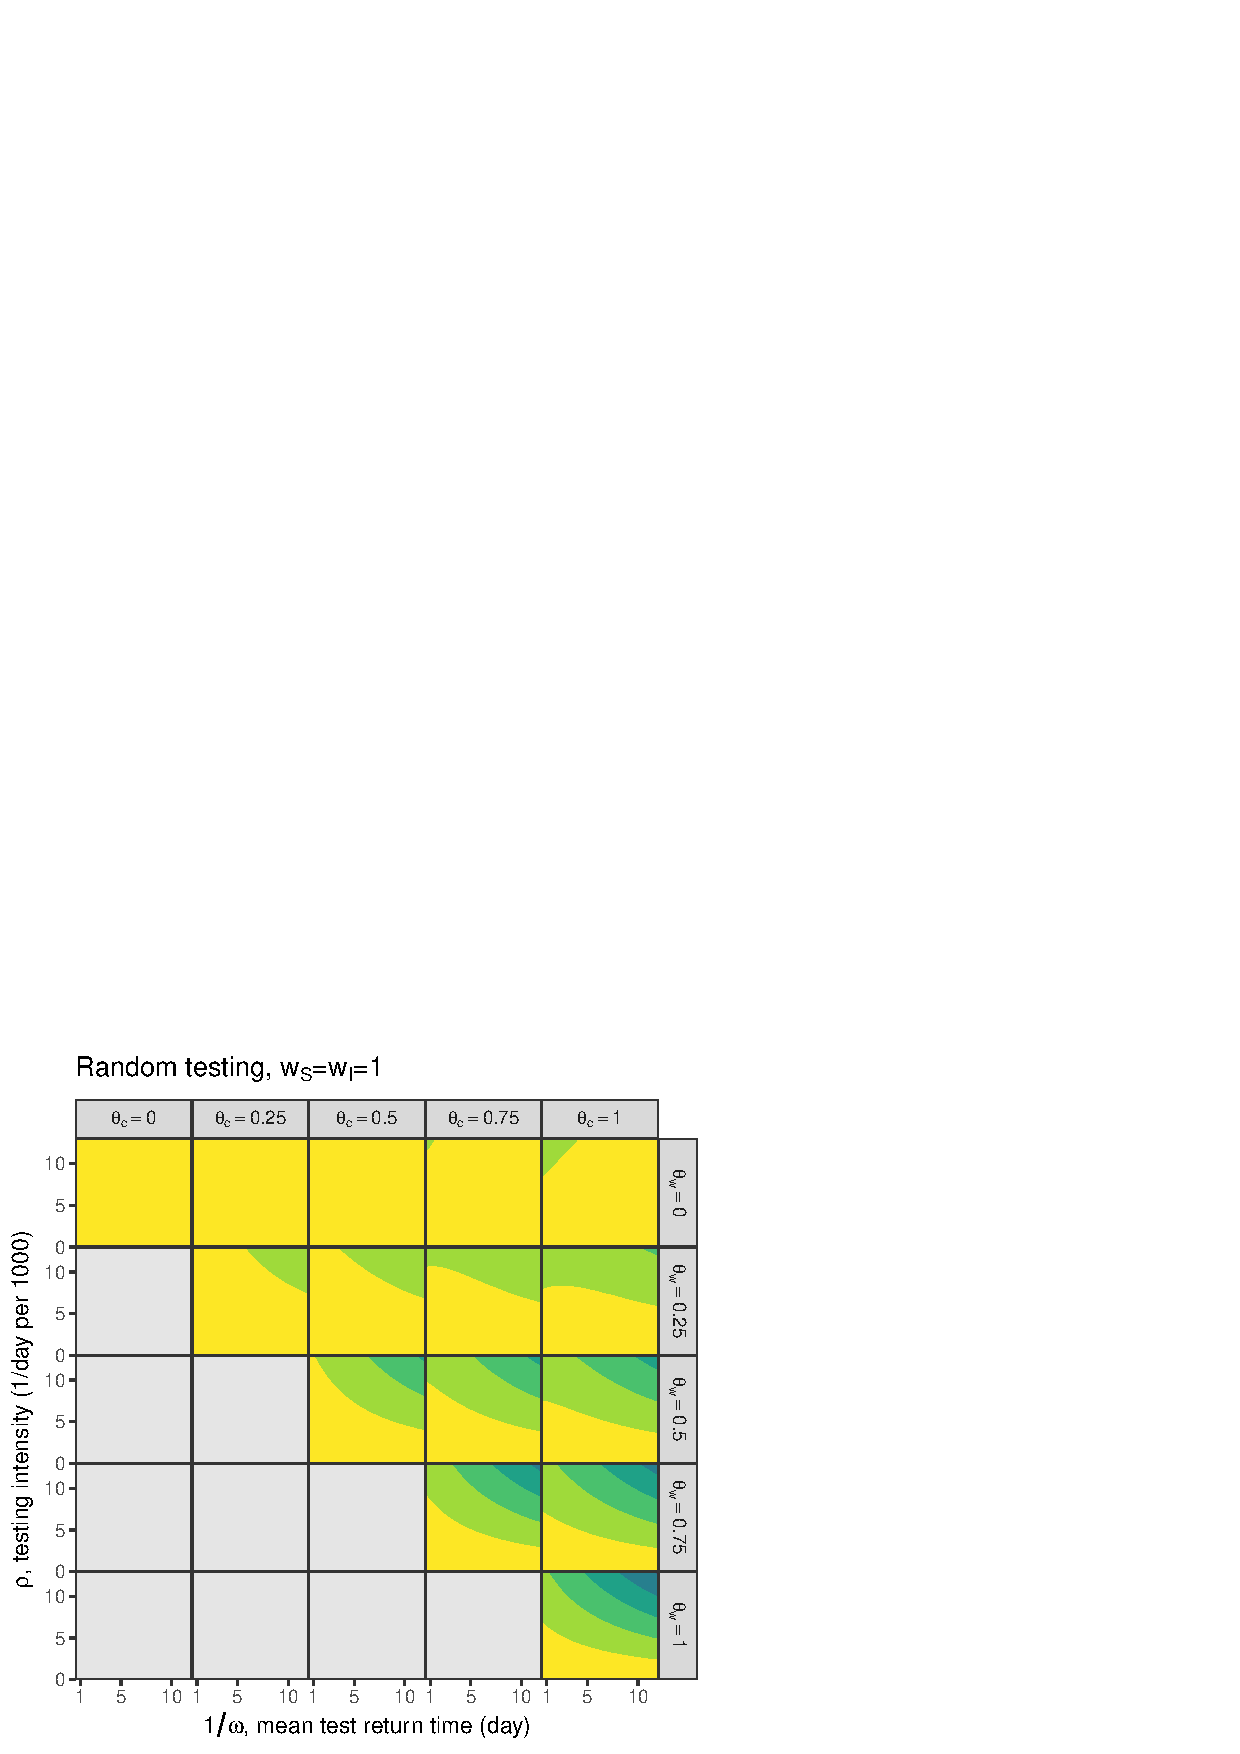
\includegraphics[width=\linewidth]{./pix/R0contour_random.png}
\end{subfigure}
%
\begin{subfigure}[t]{.45\textwidth}
\centering
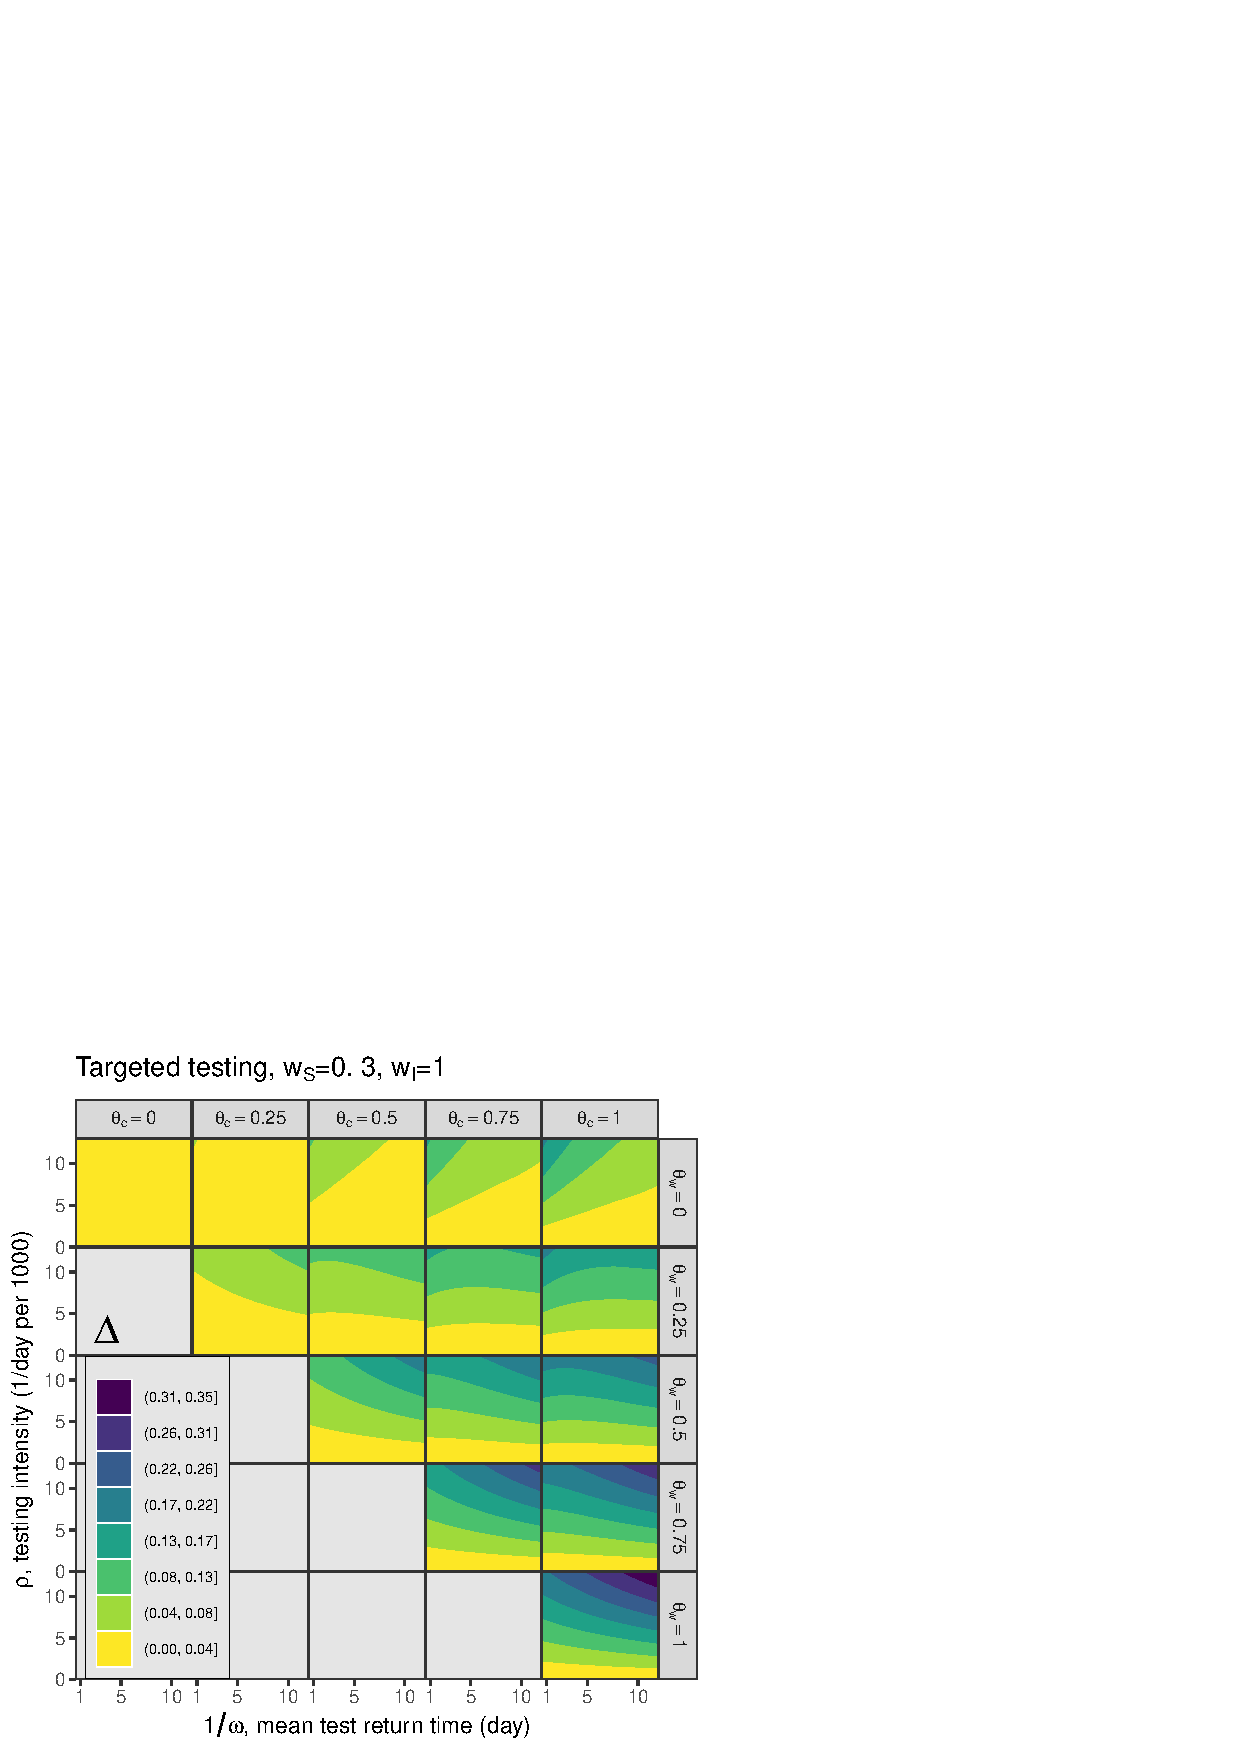
\includegraphics[width=\linewidth]{./pix/R0contour_TTI.png}
\end{subfigure}
\caption{Behaviour of the basic reproduction number, $\Rnum$, with respect to changes in the underlying parameters; remind the reader about the parameters and their values in this simulations.}
\label{fig:panels}
\end{figure}

\subsection{rate of returning tests}
The linearization of $\Rnum$ around $\rho=0$ is
\begin{equation}\label{linearization}
\Rnum \approx \beta/\gamma + \frac{\beta \rho}{\omega (\omega+\gamma) \gamma^2 W_s} \Big(\gamma(\eta_w-1)(\gamma W_s+\omega W_i) + (\eta_t -1)P_iW_i \omega^2 \Big). 
\end{equation}

So when $\rho \approx 0$ we have $$\partial{\Rnum}/\partial{\omega} \approx  \frac{-\beta \rho}{\gamma W_s\omega^2 (\gamma+\omega)^2}  (a \omega^2 + b \omega + c).$$

where $a=(\eta_w-1)W_i-(\eta_t-1)P_iW_i$, $b=2(\eta_w-1)\gamma W_s$ and $c=(\eta_w-1)\gamma^2 W_s$. 

Perhaps counter-intuitively, the equation above does not predict that $\Rnum$ is monotone decreasing with respect to $\omega$. In other words; our model does not predict that returning test results more rapidly \textit{always} lower $\Rnum$. In order to gain insight into this intriguing behaviour, we examine the zeroes of $\frac{\partial{\Rnum}}{\partial{\omega}}(\omega)$.

Defining the following quantity, $Q$, will help us write the roots of $\partial{\Rnum}/\partial{\omega}$ neatly. 
\begin{align}\label{eq:defQ}
    Q =& \frac{W_i}{W_s}\left(1-\frac{n_{t}-1}{n_{w}-1}P_{i}\right) \\
\end{align}

With that in mind, we can write the roots of $\partial{\Rnum}/\partial{\omega}$ as

\begin{align}
    \omega_1 =& \frac{\gamma}{-\sqrt{1-Q}-1} \\
    \omega_2 =& \frac{\gamma}{\sqrt{1-Q}-1}
\end{align}

Note that the zeroes are real if and only if $Q < 1$. Note that have $\eta_t < \eta_w$, so if $P_i \approx 1$, we will have $Q < 0 < 1$. Thus, if we assume near-perfect test sensitivity, $\omega_1$ and $\omega_2$ will be real. 

Assuming $\omega_1, \omega_2$ are real, it is easy to confirm that $\omega_1 < 0$ by looking at the denominator. To see that $\omega_2 > 0$, recall that $Q < 0$, so $\sqrt{1-Q} > 1$ and so $\sqrt{1-Q} -1 > 0$. Knowing that $\omega_1 < 0$, the only root of interest (i.e., biologically relevant quantity) is $\omega_2$. 

We can prove that $\partial{\Rnum}/\partial{\omega} > 0$ when $\omega \in (0,\omega_2)$ and $\partial{\Rnum}/\partial{\omega} < 0$ when $\omega \in (\omega_2,\infty)$ by computing the limits of $\partial{\Rnum}/\partial{\omega}$ at $0$ and $\infty$ respectively. So it follows that $\Rnum$ has a global maximum with respect to $\omega$ at $\omega = \omega_2$.

Now we want to characterize the parameter regions on which $\partial{\Rnum}/\partial{\omega} < 0$ (i.e., the conditions under which returning test results more rapidly is favourable). By the previous analysis, this is equivalent to solving for $\omega > \omega_2$. So

\begin{align}\label{eq:necsuf}
    &\omega > \omega_2 \nonumber \\
    &\omega > \frac{\gamma}{\sqrt{1-Q}-1} \nonumber \\
    &\vdots \nonumber \\
    &\frac{1-n_{t}}{1-n_{w}}P_{i}>\frac{W_{s}}{W_{i}}\left(\frac{\gamma}{\omega}+1\right)^{2}
\end{align}

This inequality quantifies the exact relationships between model parameters that result in returning tests more rapidly being favourable. To give a biological interpretation, we describe the qualitative \textit{trends} predicted by the inequality. Returning test results more rapidly \textit{tends} to be more favourable when

\begin{itemize}
    \item individuals who have tested positive lower their contact much more than individuals who are waiting for their test results (i.e., $\eta_t \ll \eta_w$).
    \item the test is sensitive.
    \item testing of infected individuals is more intense than testing of susceptible individuals.
\end{itemize}
An in-depth discussion of these results is presented in the discussion section. 

\subsection{Expensive vs. cheap tests}

The use of tests cheaper than RT-PCR has been proposed as a potential strategy for containing the COVID-19 pandemic. While cheaper tests may be less sensitive and reliable than RT-PCR, they allow for broader and more intense testing. In the analysis below, we compare the $\Rnum$ predicted by our model depending on the testing strategy. 

Consider a test that allows us to test at rate $\rho_1$ and has sensitivity $P_{i,1}$, and another test that allows us to test at $\rho_2$ and has sensitivity $P_{i,2}$. Suppose that $\rho_1 > \rho_2$. Recall that the linearization of $\Rnum$ around $\rho \approx 0$ is given by $$\Rnum \approx \beta/\gamma + \frac{\beta \rho}{\omega (\omega+\gamma) \gamma^2 W_s} \Big(\gamma(\eta_w-1)(\gamma W_s+\omega W_i) + (\eta_t -1)P_iW_i \omega^2 \Big).$$


Treating $\Rnum$ as a function of $\rho$ and $P_i$,we can reduce the inequality $$\Rnum(\rho_2, P_{i,2}) < \Rnum(\rho_1, P_{i,1})$$ into 

\begin{align}\label{eq:rho1vsrho2}
    &\rho_1\left(\gamma(\eta_w-1)(\gamma W_s + \omega W_i) + (\eta_t-1)P_{i, 1}W_i\omega^2\right) - \rho_2\left(\gamma(\eta_w-1)(\gamma W_s + \omega W_i) + (\eta_t-1)P_{i, 2}W_i\omega^2\right) > 0 \nonumber \\
    &\vdots \nonumber \\
    &\frac{\rho_2P_{i, 2}-\rho_1P_{i, 1} }{\rho_1-\rho_2} > \frac{1-\eta_w}{1-\eta_t}\cdot \frac{\gamma(\gamma W_s + \omega W_i)}{\omega^2 W_i}
\end{align}

Note that the RHS is positive, thus a necessary condition for the inequality above to hold is that $\rho_2P_{i,2} > \rho_1P_{i,1}$, equivalently 

\begin{equation}
\frac{P_{i,2}}{P_{i,1}} > \frac{\rho_1}{\rho_2}.
\end{equation}

To state an example of this, if test $A$ is three times as expensive as test $B$ (and hence one can test three times as many people with test $B$), using test $A$ rather than $B$ will be favourable only if test $A$ is at least 3 times more sensitive than test $B$. Note that this is a necessary but not sufficient condition, so even if test $A$ is three times more sensitive, it is still possible for test $B$ to be more effective. 

\cref{eq:rho1vsrho2} tells us precisely when a test corresponding to $\rho_2, P_{i,2}$ will yield a lower $\Rnum$ than a test corresponding to $\rho_1, P_{i,1}$, where $\rho_1 > \rho_2$. Some of the qualitative \textit{trends} that favour test 2 (the higher-sensitivity test) include

\begin{itemize}
    \item individuals who test positive self-isolate much more than individuals who are waiting for their test result.
    \item the time it takes to return tests is much shorter than the mean infectious period.
    \item the testing intensity is much greater for infected individuals than susceptible individuals.
\end{itemize}

% %%%%%%%
\section{Discussion}

- JD's email:
We're basically looking at the potential advantage of slow tests:
people waiting for test results may be more careful than those who
have received negatives. These advantages are real, and neglected. We
also compare to an individual-level advantage of fast tests: people
who test positive may be even more careful. But we are missing out on
community-level advantages of fast testing: better assessment of the
situation, identification of hot spots, contact-tracing, etc. 

- May be something about the testing rate/intensity, now the per capita testing intensity is very low ($\rho \approx 0$). In near future new test kits may be widely accessible, our model provide insights in this case (what are those?)

- "delay negative results" result

\subsection{Rate of returning tests}
\fady{needs to be expanded}
When the difference in self-isolation between individuals waiting for their tests and individuals who are confirmed positive is small, returning tests rapidly is not beneficial because the benefit in doing so (i.e., the extra self-isolating when an individual tests positive) is minimal and outweighed by the fact that those who test negative may increase their contacts. Similarly, if the test is not sensitive, many infected individuals will test negative, and thus may increase their contacts under the false belief that they are not infectious, hence returning test results more quickly in this case may not be beneficial. 

When testing of infected individuals is more intense than susceptible individuals, returning test results rapidly is beneficial because those infected individuals will be informed and self-isolate. Conversely, if testing of susceptible individuals is much greater, very few tests be positive, and the benefit of informing those few positive cases will be outweighed by the potential increase in contacts of the individuals testing negative. 

\subsection{Expensive vs. cheap tests}
\fady{needs to be written \dots must discuss the fact that our analysis holds only when $\rho$ is relatively small, so if there is a test so cheap that $\rho$ does not stay small, our results do not apply.}


% %%%%%%%
\bibliography{SIRlibrary.bib}

% %%%%%%%
\section{supplementary material}

The next generation matrix, $G = F V^{-1}$, is in the lower triangular form with $F$ and $G$ as follows.


\begin{equation}\label{FV}
F= \beta/N_0 \left[ \begin {array}{cccc} 
S_u&\eta_w\,S_u&\eta_w\,S_u&\eta_t\,S_u\\
S_n&\eta_w\,S_n&\eta_w\,S_n&\eta_t\,S_n\\ 
0&0&0&0\\
0&0&0&0
 \end {array} \right],
 V=
 \left[ \begin {array}{cccc}  
F_I+\gamma&-\omega&0&0\\
-(1-p_I)F_I&\omega+\gamma&0&0\\
-p_I F_I&0&\omega+\gamma&0\\
0&0&-\omega&\gamma
\end {array} \right],
\end{equation}

\begin{equation}
G = \left[ \begin {array}{cc}
G_{11}&G_{12}\\
0&0
\end {array} \right], \text{ where } \\
G_{11} =C
\left[\begin {array}{cc}
A\,S_u & B\,S_u\\
A\,S_n & B\,S_n
\end {array}\right],
\end{equation}

The Eigenvalues of $G_{11}$, are 0 and $\Rnum$.

% %%%%%%%
\section{Literature Review}

\subsection{Explicit models of TTI (trace/test/isolate) based on network or agent-based models}
\citep{endo2020implication} [Ali: It seems to me that this is just a statistical model to estimate the parent-offspring of an infected index, not sure if it fits into agent-based group!] Used simulation on a branching process model to assess the forward and backward contact tracing efficiency. Assuming a negative-binomial branching process with a mean R, reproduction number, and overdispersion parameter k, the mean total number of generation G3 and averted G3 are estimated. The effectiveness of TTI is defined as the ratio of averted to the mean.

\citep{jenness2020modeling} developed a network-based transmission model for SARS-CoV-2 on the Diamond Princess outbreak to characterize transmission dynamics and to estimate the epidemiological impact of outbreak control and prevention measures. 

\citep{elbanna2020entry} [seems similar to MacPan model!]

\citep{de2020influenza} Was discussed in the Math 747 
SEIR Asymptomatic and symptomatic $I_1, I_2$. Used linear chain trick 
Stringency index as a control force lowering $\beta$.

\citep{rice2020effect} Effect of school closures on mortality. Reproduce Report 9 results by spatial agent based CovidSim. 
% %%%%%%%
\subsection{Models of repeated random testing of isolated populations}
\cite{bergstrom2020frequency}
(1) Model, assumptions: They developed a function, namely expected exposure $E(C,\tau)$, to approximate trade-offs between the frequency of testing, n, the sensitivity of testing, q, and the delay between
testing and results, d. This function is explicitly derived and was connected the effective reproduction number $R=R_0 S$, where $S$ is the proportion of population susceptible.
assumption that transmission rates are a step function: individuals who
have COVID go from non-infectious to fully infectious instantaneously,
and remain fully infectious until they are no longer able to transmit disease. Test sensitivity takes the same form over the course of infection.
More sophisticated models could allow varying infectiousness and varying
sensitivity over time, as in 
\citep{larremore2020test}.

\citep{lopman2020model} Used a Deterministic SEIR model, incorporated TTI, applicable to a university setting. They assumed a fairly high reproductive number that is not reduced through social
distancing measures. They found that community-introduction of SARS-CoV-2 infection onto campus can be
relatively controlled with effective testing, isolation, contract tracing and quarantine.

\citep{tuite2020mathematical} used an age-structured compartmental model of COVID-19 transmission in the population of Ontario, Canada. We compared a base case with limited testing, isolation and quarantine to different scenarios. 
% %%%%%%%
\subsection{Other maybe-related works}
\citep{arino2020simple} developed a SLIAR compartmental model to study the spread of an epidemic, specifically COVID-19, in a population. The model incorporates an Erlang distribution of times of sojourn in incubating, symptomatically and asymptomatically infectious compartments. Basic reproduction number is derived. Also, sensitivity analysis with respect to the underlying parameters for the following two outputs was carried out; (i) the number of observable cases during the course of the epidemic and at the peak, and (ii) the timing of the peak of the outbreak. Sensitivity analysis is performed using the R package multisensi.

\citep{ruszkiewicz2020diagnosis} novel with-in-a-minute breath testing with 80\% accuracy. 


\end{document}






